% ncse_new/p2_InterpolationApproximation/ch4_NumericalQuadrature/ex_QuadraturePlots.tex
% exercise requires:   ExQuadPlots.jpg     ExQuadPlots.eps
% solutions require:   -

\begin{problem}[Quadrature plots] \label{prb:QuadraturePlots}

We consider three different functions on the interval $I=[0,1]$:
\begin{align*}
\text{function A:}\quad f_A&\in \text{analytic}\;,\quad f_A\notin\Cp_k\; \forall\;k\in\IN\;;\\
\text{function B:}\quad f_B&\in C^0(I)\;,\quad f_B\notin C^1(I)\;;\\
\text{function C:}\quad f_C&\in\Cp_{12}\;,
\end{align*}
where $\Cp_k$ is the space of the polynomials of degree at most $k$ defined on $I$.
The following quadrature rules are applied to these functions:
\begin{itemize}
\item quadrature rule A,\quad global Gauss quadrature;
\item quadrature rule B,\quad composite trapezoidal rule;
\item quadrature rule C,\quad composite 2-point Gauss quadrature.
\end{itemize}
The corresponding absolute values of the quadrature errors are plotted against the number of function evaluations in Figure~\ref{fig:QuadraturePlots}.
Notice that only the quadrature errors obtained with an even number of function evaluations are shown.

\begin{figure}[hbt]
\hspace{8mm}
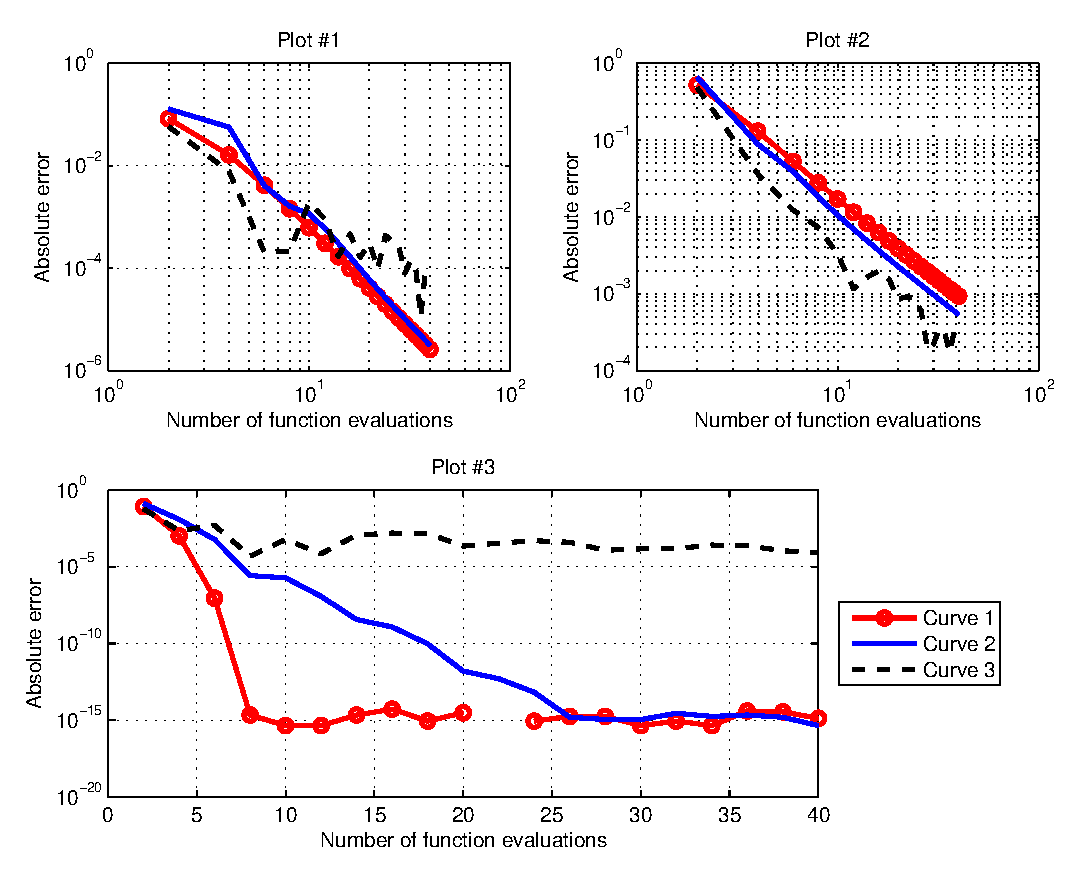
\includegraphics[width=0.9\textwidth]{\problems/ch_numericalquadrature/PICTURES/ExQuadPlots.eps}
\caption{Quadrature convergence plots for different functions and different rules.}
\label{fig:QuadraturePlots}
\end{figure}

%%%%%%%%%%%% SUBPROBLEM 1

\begin{subproblem}[3] \label{prb:QuadraturePlots_1}
Match the three plots (plot \#1, \#2 and \#3) with the three quadrature rules (quadrature rule A, B, and  C). Justify your answer.\\[1.5ex]
\begin{hint}
Notice the different axis scales in the plots.
\end{hint}

\begin{solution}
Plot \#1 --- Quadrature rule C, Composite 2-point Gauss:\\
algebraic convergence for every function, about $4^{th}$ order for two functions.

Plot \#2 --- Quadrature rule B, Composite trapezoidal:\\ algebraic convergence for every function, about $2^{nd}$ order.

Plot \#3 --- Quadrature rule A, Global Gauss:\\ algebraic convergence for one function, exponential for another one, exact integration with 8 evaluations for the third one.
\end{solution}
\end{subproblem}

%%%%%%%%%%%% SUBPROBLEM 2

\begin{subproblem}[3] \label{prb:QuadraturePlots_2}
The quadrature error curves for a particular function $f_A$, $f_B$ and $f_C$ are plotted in the same style (curve 1 as red line with small circles, curve 2 means the blue solid line, curve 3 is the black dashed line).
Which curve corresponds to which function ($f_A$, $f_B$, $f_C$)?
Justify your answer.

\begin{solution}
Curve 1 red line and small circles --- $f_C$ polynomial of degree 12:\\
integrated exactly with 8 evaluations with global Gauss quadrature.

Curve 2 blue continuous line only --- $f_A$ analytic function:\\
exponential convergence with global Gauss quadrature.

Curve 3 black dashed line --- $f_B$ non smooth function:\\
algebraic convergence with global Gauss quadrature.
\end{solution}
\end{subproblem}
\end{problem}
